\documentclass{standalone}
\usepackage{tikz}
\usepackage{pgfplots}
\pgfplotsset{width=32cm,height=18cm,compat=1.3}
\pgfplotsset{every tick label/.append style={font=\Huge}}
\usepackage{filecontents}

\usetikzlibrary{patterns}

\definecolor{citrine}{rgb}{0.89, 0.82, 0.04}

\begin{document}
	\centering
		\vspace{1.5em}
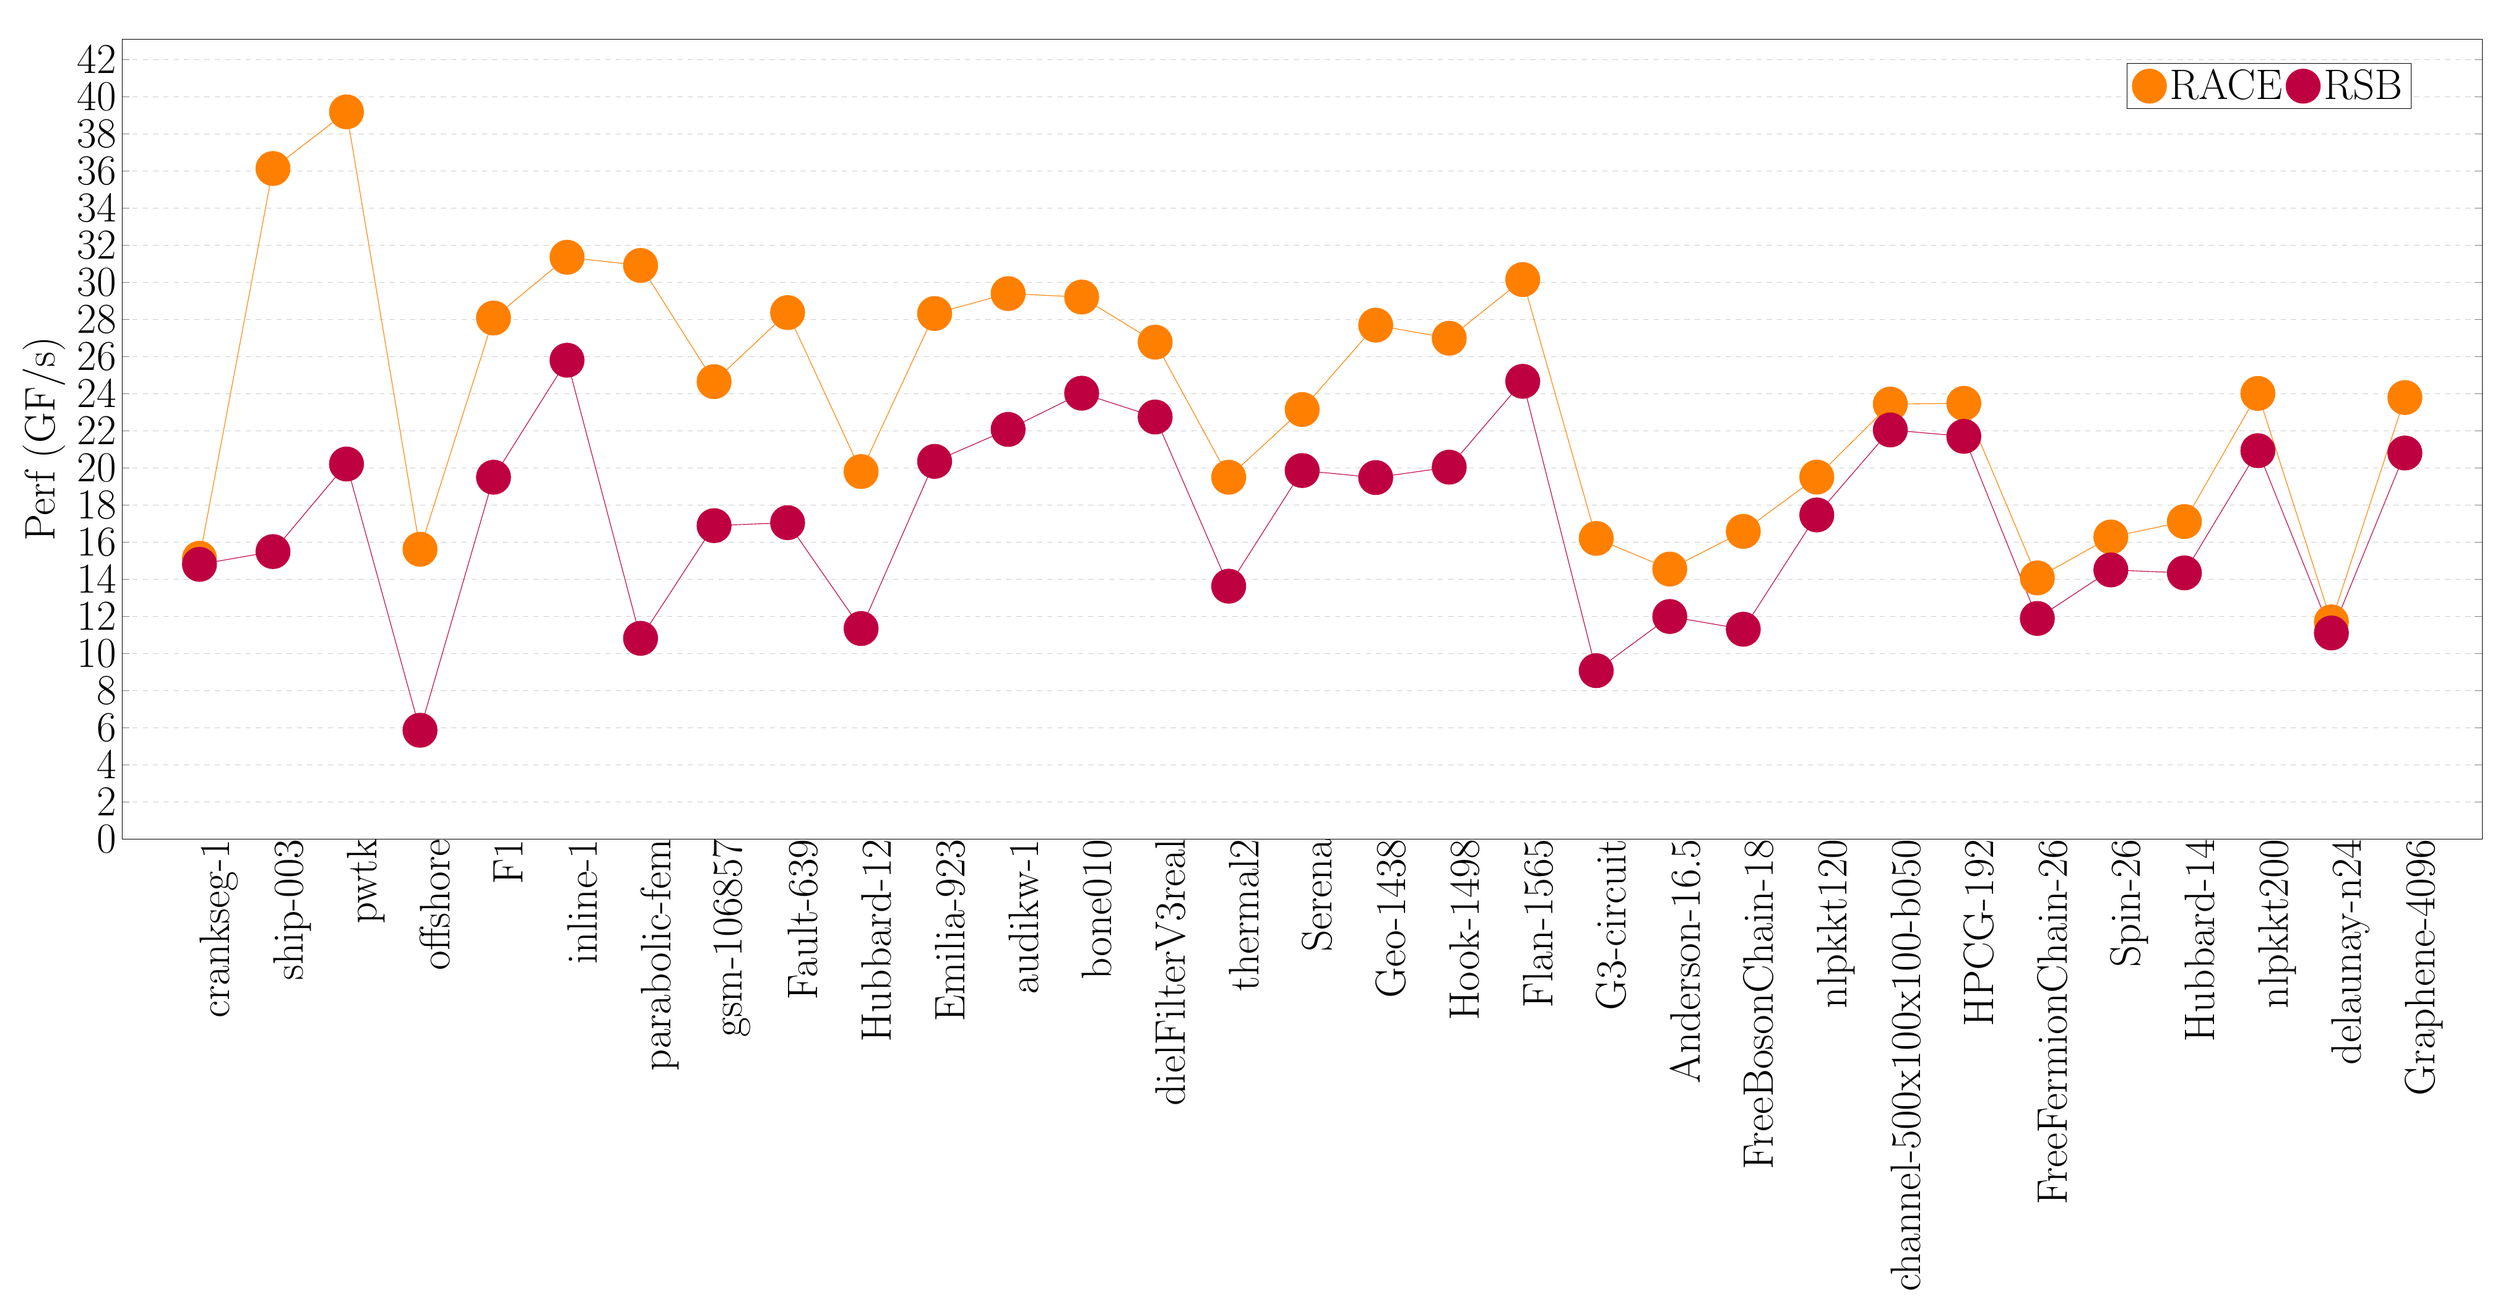
\begin{tikzpicture}
		%	\node at (13.25,15) {\LARGE{}};
			\begin{axis}[
		%	xmin=0.25, xmax=7.25,
			ymin=0, %ymax=3.25,
			xtick={1, 2, 3, 4, 5, 6, 7, 8, 9, 10, 11, 12, 13, 14, 15, 16, 17, 18, 19, 20, 21, 22, 23, 24, 25, 26, 27, 28, 29, 30, 31},
		%	ytick={0,0.5,1,1.5,2,2.5,3},
			xticklabels={crankseg-1, ship-003, pwtk, offshore, F1, inline-1, parabolic-fem, gsm-106857, Fault-639, Hubbard-12, Emilia-923, audikw-1, bone010, dielFilterV3real, thermal2, Serena, Geo-1438, Hook-1498, Flan-1565, G3-circuit, Anderson-16.5, FreeBosonChain-18, nlpkkt120, channel-500x100x100-b050, HPCG-192, FreeFermionChain-26, Spin-26, Hubbard-14, nlpkkt200, delaunay-n24, Graphene-4096},
			width  = 50cm,
			height = 18cm,
			major x tick style = transparent,
			%	minor ytick={1, 5, 10, 15, 20, 25, 30 ,35,40},
			grid = minor,	
			%add_bar_commands
			ymajorgrids = true,
			grid style={dashed, gray!40},
			ylabel = {\Huge{Perf (GF/s)}},
		%	symbolic x coords={Graphene-2048-2048, Graphene-4096-4096, Spin-24-24-24},
			x tick label style={rotate=90, anchor=north east, inner sep=0mm, font={\Huge}},
			tick label style={font={\Huge}},
			scaled y ticks = false,
			enlarge x limits=0.035,
			legend cell align=left,
			legend style={font=\Huge},
			legend columns=-1,
			legend style={
				%at={(1,1.05)},
				%anchor=south east,
				%column sep=1ex,
				legend pos=north east
			},
			%spl_legend_code
			title= {\Huge\scalebox{1.5}{{}}}
			]

\addplot[ mark=*, mark size=10pt, mark options={orange}, draw=orange ] plot coordinates{(1,15.130207) (2,36.140175) (3,39.194893) (4,15.613967) (5,28.080251) (6,31.356939) (7,30.913152) (8,24.649314) (9,28.372987) (10,19.802304) (11,28.323231) (12,29.396679) (13,29.210280) (14,26.778583) (15,19.496395) (16,23.148677) (17,27.696097) (18,26.990050) (19,30.152423) (20,16.199662) (21,14.545610) (22,16.577436) (23,19.505411) (24,23.441453) (25,23.480804) (26,14.069287) (27,16.275497) (28,17.107030) (29,24.014713) (30,11.700657) (31,23.793009)};
\addplot[ mark=*, mark size=10pt, mark options={purple}, draw=purple ] plot coordinates{(1,14.799869) (2,15.488695) (3,20.209989) (4,5.855544) (5,19.498048) (6,25.804495) (7,10.812407) (8,16.887582) (9,17.047021) (10,11.340355) (11,20.351504) (12,22.073317) (13,24.026902) (14,22.743862) (15,13.623255) (16,19.857215) (17,19.478608) (18,20.040225) (19,24.667225) (20,9.070211) (21,11.989002) (22,11.302683) (23,17.463520) (24,22.047775) (25,21.700950) (26,11.883824) (27,14.499154) (28,14.340057) (29,20.929050) (30,11.101159) (31,20.801896)};
	%addplot cmd

	\legend{RACE, RSB}

	\end{axis}			
\end{tikzpicture}

\end{document}

